
\noindent {\bf Challenge Problem.}
Fluid flow and heat removal through fuel, shield and reflector assemblies  can
have major impacts on operation and safety for Sodium Fast Reactors (SFRs).
This type of reactor is of great interest in the United States due to the
planned  deployment of Terrapower's Natrium concept funded partially through
the Advanced Reactor Demonstration program (ARDP). These assemblies are formed
by bundles from 19 to 217 pins, with a wire wrapped around each pin to maintain
the rods in place.

\begin{wrapfigure}{rt}{3.2in} \centering
   {\setlength{\unitlength}{1.0in} \begin{picture}(3.000,1.850)(0.05,.14)
     \put(0,0.00){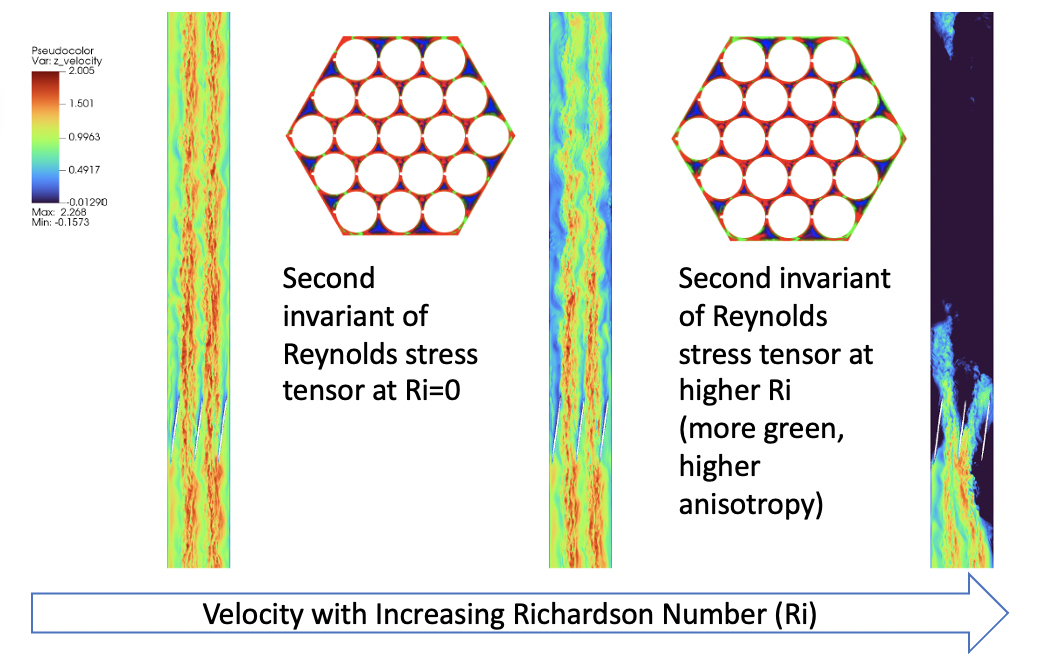
\includegraphics[scale=0.43]{figs/challenge.png}}
   \end{picture}} 
   \caption{Velocity distribution in wire-wrapper assembly as a function of
    the Richardson number at low flow conditions. \label{fig:cha}} 
\end{wrapfigure}
During transients these assemblies are characterized by a range of conditions
due to the reduced flow rates and large-scale organized flow patterns,
including potential intra-assembly buoyancy-driven circulation. Such low flow
cases can provide challenges for experiments due to complications in measuring
the flow rates and temperatures with high accuracy in different areas. This
consequently also raises the uncertainty of many modeling approaches for these
phenomena, where existing correlations and sub-channel methods fail. An example
of the complex range of flow patterns in provided in Figure~ which shows a
transition from steady forced convection to mixed convection. Massive
circulations are introduced: in a realistic transient the bundle will encounter
the full range of conditions. We ultimately seek methods that can provide
accurate and \textit{predictive} results.

% \begin{figure}[t!] \centering
%     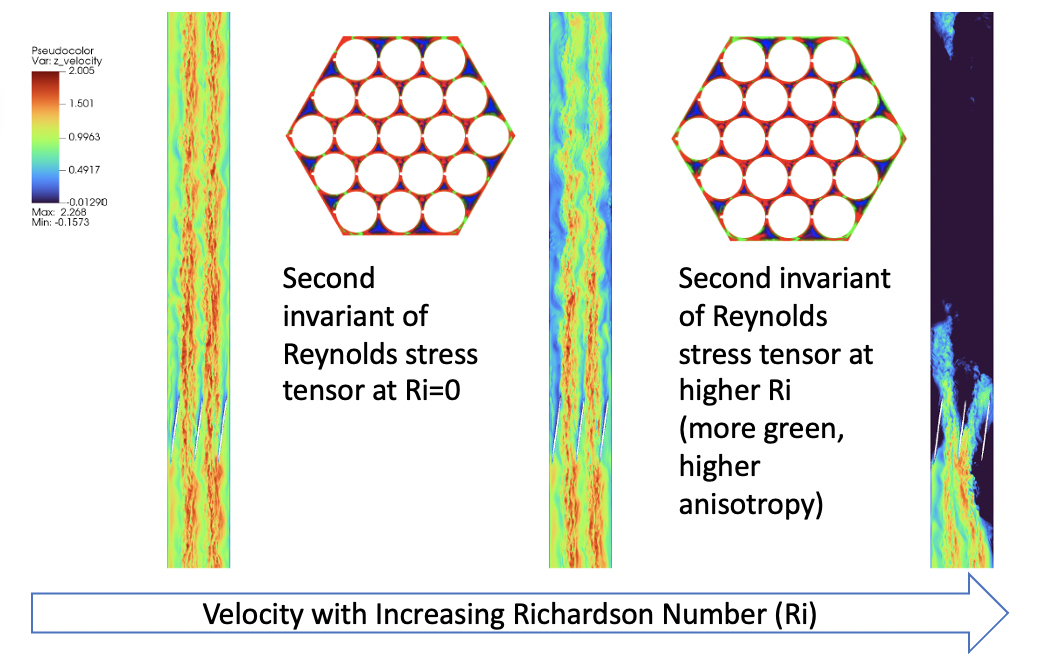
\includegraphics[width = 0.50\textwidth]{figs/challenge.png}
%     \caption{ Velocity distribution in wire-wrapper assembly as a function of
%     the Richardson number at low flow conditions. \label{fig:cha}} 
% \end{figure}

